\documentclass[12pt]{article}

\usepackage{sbc-template}
\usepackage{graphicx,url}
\usepackage[utf8]{inputenc}
\usepackage[brazil]{babel}
     
\sloppy

\title{Relatório da Implementação do módulo
	de cadastro de questionário }

\author{
	Cristian Diamantaras Vilela\inst{1},
	Filipe Castelo Branco de Souza\inst{1},\\
	Gabriel da Fonseca Ottoboni Pinho\inst{1},
	João Pedro Cavalcante Mateus da Silva\inst{1},\\
	Rodrigo Delpreti de Siqueira\inst{1}
}


\address{Instituto de Computação --
	Universidade Federal do Rio de Janeiro (UFRJ)\\
}

\begin{document} 

\maketitle

\begin{abstract}
  This report describes a web project implementation
  to be used in form registry, in accordance to the
  VODAN BR support database schemas.
\end{abstract}
     
\begin{resumo} 
  Este relatório descreve a implementação
  de um projeto web
  para cadastro de formulário,
  segundo requisitos da base de dados
  de apoio VODAN BR.
\end{resumo}

\section{Introdução}

No desenvolvimento da implementação
apresentada no presente relatório,
utilizaram-se as frameworks React e Laravel
para o desenvolvimento do front-end e back-end
respectivamente.
Tais escolhas foram baseadas no conhecimento prévio
da equipe, bem como no interesse de aprendizado dos membros.

O código está disponibilizado no repositório do
Github: \url{https://github.com/gabrielott/bd-final}.

\section{Interface} \label{sec:firstpage}

A interface da aplicação visa a montagem
dos questionários à partir de botões e dropdowns,
estruturados conforme a hierarquia designada na especificação.
Estes componentes podem ser visualizados nas imagens abaixo.

\begin{figure}[ht]
	\centering
	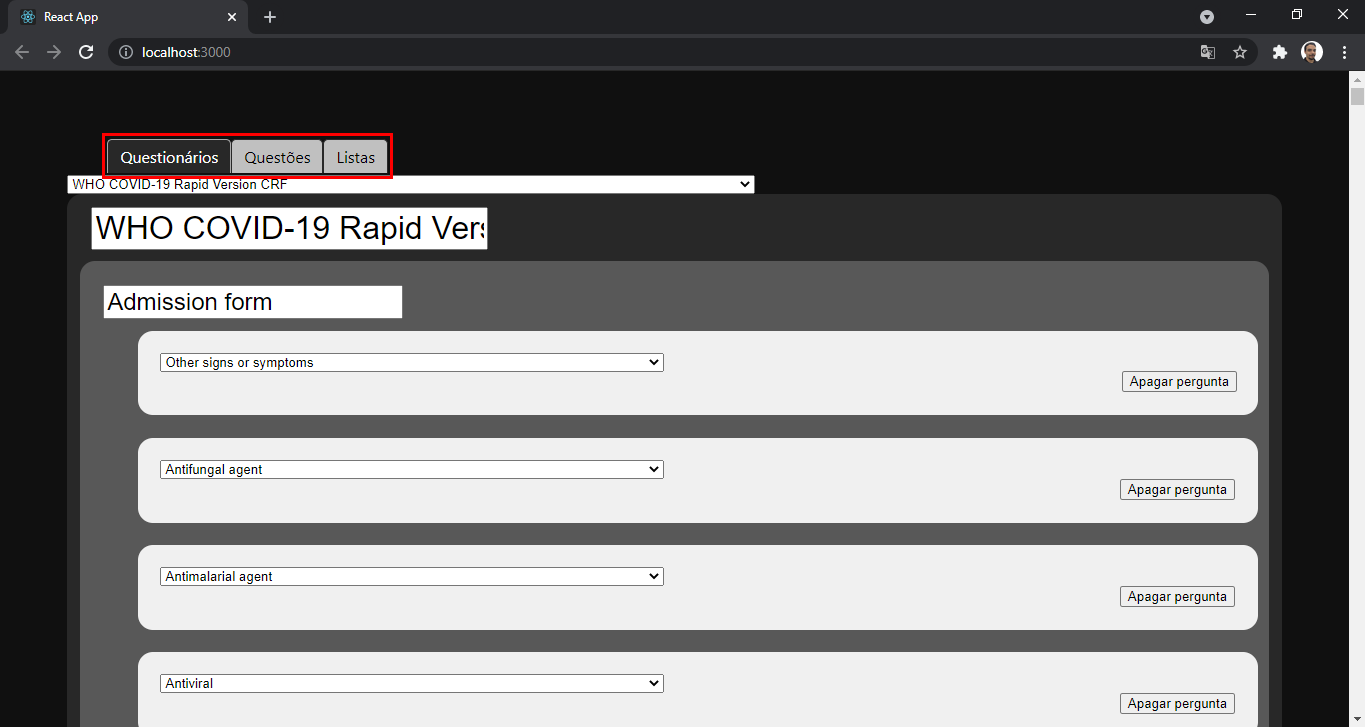
\includegraphics[width=.5\textwidth]{front.png}
	\caption{Interface da aplicação}
	\label{fig:Figura1}
\end{figure}

Inicialmente, as funcionalidades estão divididas nas abas
Questionários, Questões e Listas, conforme destacado
em vermelho. Na aba Questionários,
podemos observar a hierarquia proposta,
sinalizada pelos tons de cinza,
onde o formulário possui módulos, os quais possuem questões.
As opções para criar e apagar estão disponíveis,
e ao final há um botão para salvar o questionário.

\begin{figure}[ht]
	\centering
	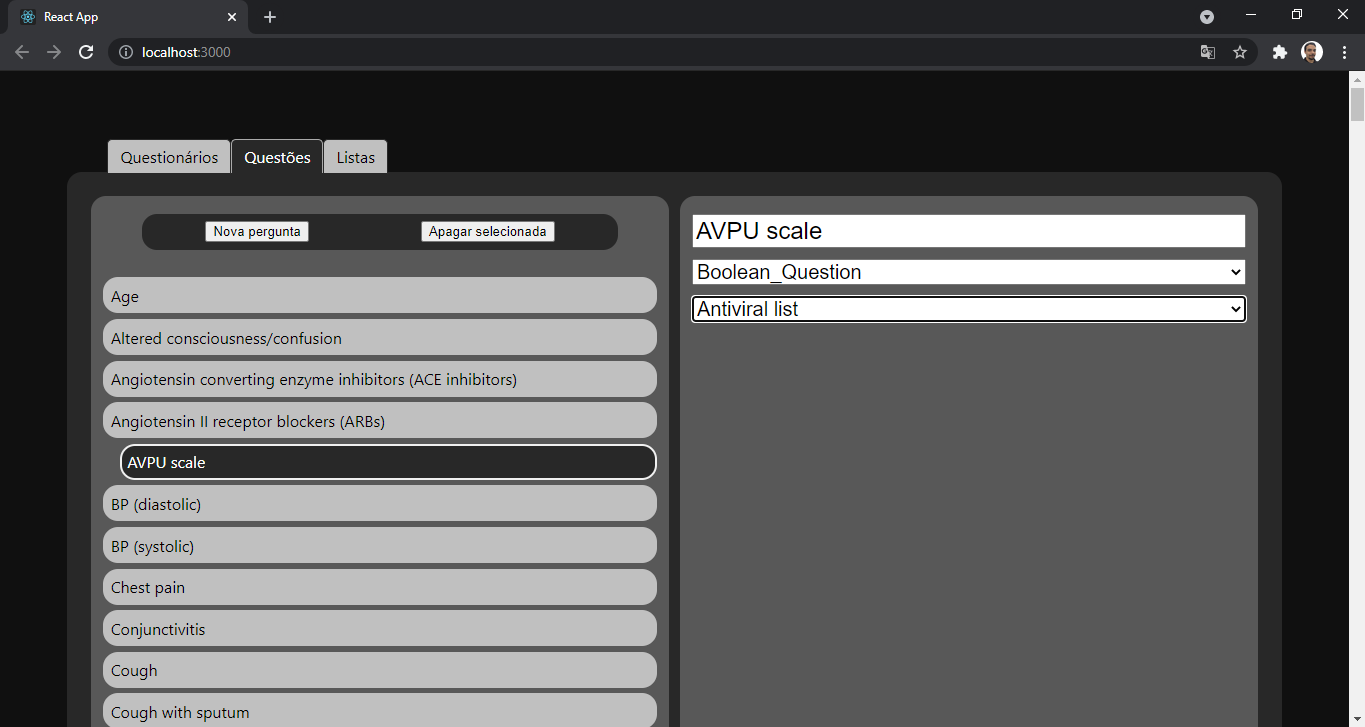
\includegraphics[width=.5\textwidth]{questoes.png}
	\caption{Aba de Questões}
	\label{fig:Figura2}
\end{figure}

\begin{figure}[ht]
	\centering
	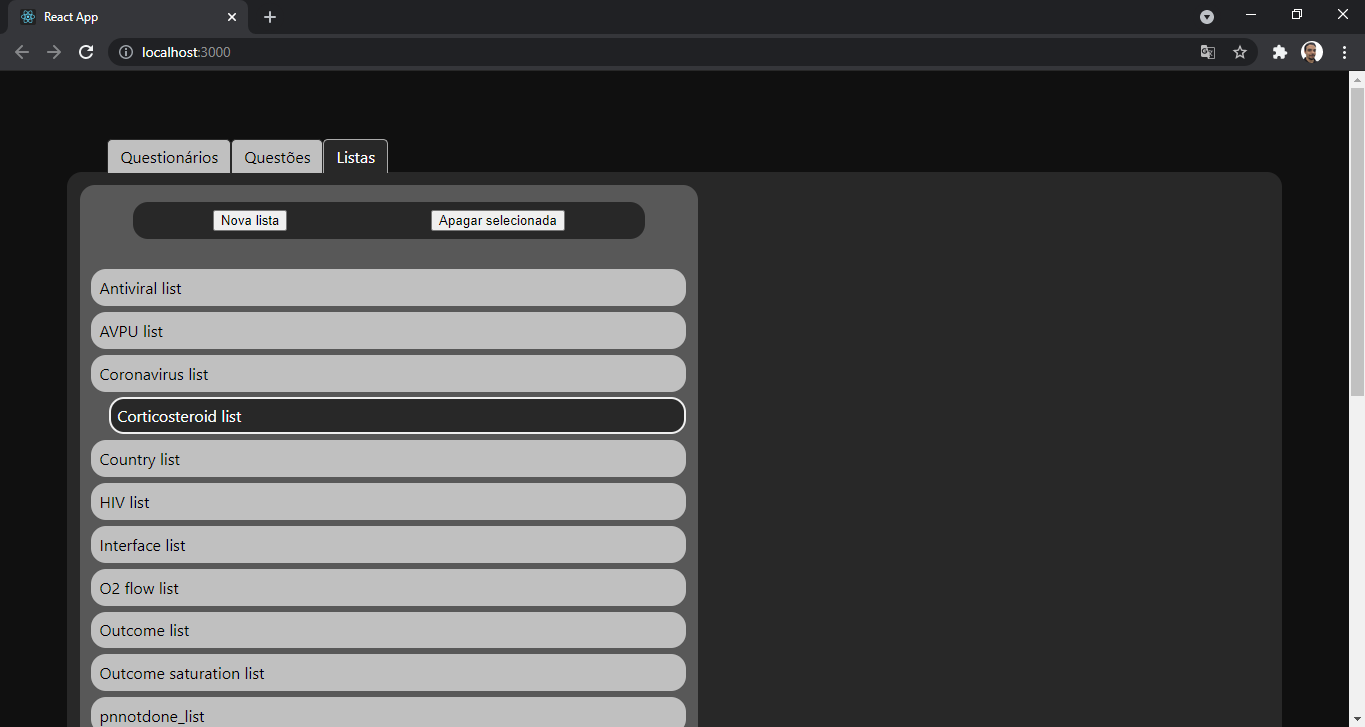
\includegraphics[width=.5\textwidth]{listas.png}
	\caption{Aba de Listas}
	\label{fig:Figura3}
\end{figure}

As abas para Questões e Listas,
conforme pode ser visto nas figuras 2 e 3,
servem para editar as mesmas.
Os botões para salvar/descartar as alterações
encontram-se na parte inferior da página.

\section{Back-end}

Para o back-end do projeto, foi utilizada
a linguagem PHP 8.0 com a framework Laravel 8.40.
O banco de dados foi armazenado em um servidor
local com Apache, MariaDB e MySQL.

Algumas mudanças foram feitas no banco
de dados original do Vodan para facilitar
o uso de chaves estrangeiras e relacionamentos.
Isso tornou os relacionamentos concisos
e os atributos levemente reduzidos.

Foi seguido o padrão de projeto MVC (Model-View-Controller),
para o reuso de código e separação de conceitos
nessas três camadas, em que Model e Controller
estão no back-end, e a View fica
no front-end da aplicação.

\subsection{Seeder}

Para simularmos o banco de dados inicial,
utilizamos sintaxe MySQL (com \texttt{DB::statement})
para inserirmos os dados nas tabelas do banco.
Foram enviados dois questionários,
\textit{WHO COVID-19 Rapid Version CRF} e
\textit{FICHA DE INVESTIGAÇÃO DE SG SUSPEITO
DE DOENÇA PELO CORONAVÍRUS 2019 – COVID-19 (B34.2)},
ambas disponibilizadas na pasta do
Google Drive com demais informações do trabalho

Grande parte já possuía um script disponibilizado,
então tivemos apenas que modificar algumas coisas
para seguir o padrão que adotamos no banco de dados
e adicionar o novo formulário com seus módulos,
questões e respostas padronizadas referentes.

\subsection{Rotas}

O arquivo \texttt{api.php} contém as rotas da nossa aplicação.
Nele encontram-se o método da requisição,
o nome da rota, o arquivo onde está a função
que será utilizada, e o nome da mesma.

O fluxo da aplicação ocorre nessa ordem:
o front-end chama uma rota no back,
que está descrita no arquivo \texttt{api.php}.
A rota está conectada a uma função em uma Controller,
que chamará uma função na Model.
Na Model ocorrerá a função e interação
com o banco de dados, que retornará
alguma requisição para o front,
dependendo da função executada.
Este é o padrão MVC comentado anteriormente.

\subsection{Controllers}

Na Controller é feita a verificação
e tratamento inicial dos parâmetros.
Estes parâmetros serão passados
para uma função na respectiva Model
e depois o retorno é enviado para o front.

\subsection{Models}

As models são os arquivos que representam
algumas funções de visualização, criação,
atualização e deleção, além de relacionamentos
entre tabelas. A vantagem de se usar o Laravel
nesses casos é utilizar as funções
de relacionamentos para fazer queries aninhadas
com uma sintaxe fácil, graças ao Eloquent ORM,
sobre o qual não entraremos em muitos detalhes.

\section{Integração}

Assim, conforme o modelo descrito acima, as páginas
apresentadas no front-end realizam requisições para a API
servida no back-end.



\section{Referências}

\cite{1}, \cite{2}, \cite{3}.

\bibliographystyle{sbc}
\bibliography{sbc-template}

\end{document}
